\documentclass{article}

\usepackage{graphicx}
\usepackage{tikz}
\usepackage{tikzsymbols}
\usetikzlibrary{calc,patterns,shapes.geometric}
\pagestyle{empty}
\usepackage[margin=0pt]{geometry}
\geometry{papersize={14in,12in}}

\def\centerarc[#1](#2)(#3:#4:#5){\draw[#1] ($(#2)+({#5*cos(#3)},{#5*sin(#3)})$) arc (#3:#4:#5);}

\begin{document}
	\begin{figure}
		\centering
		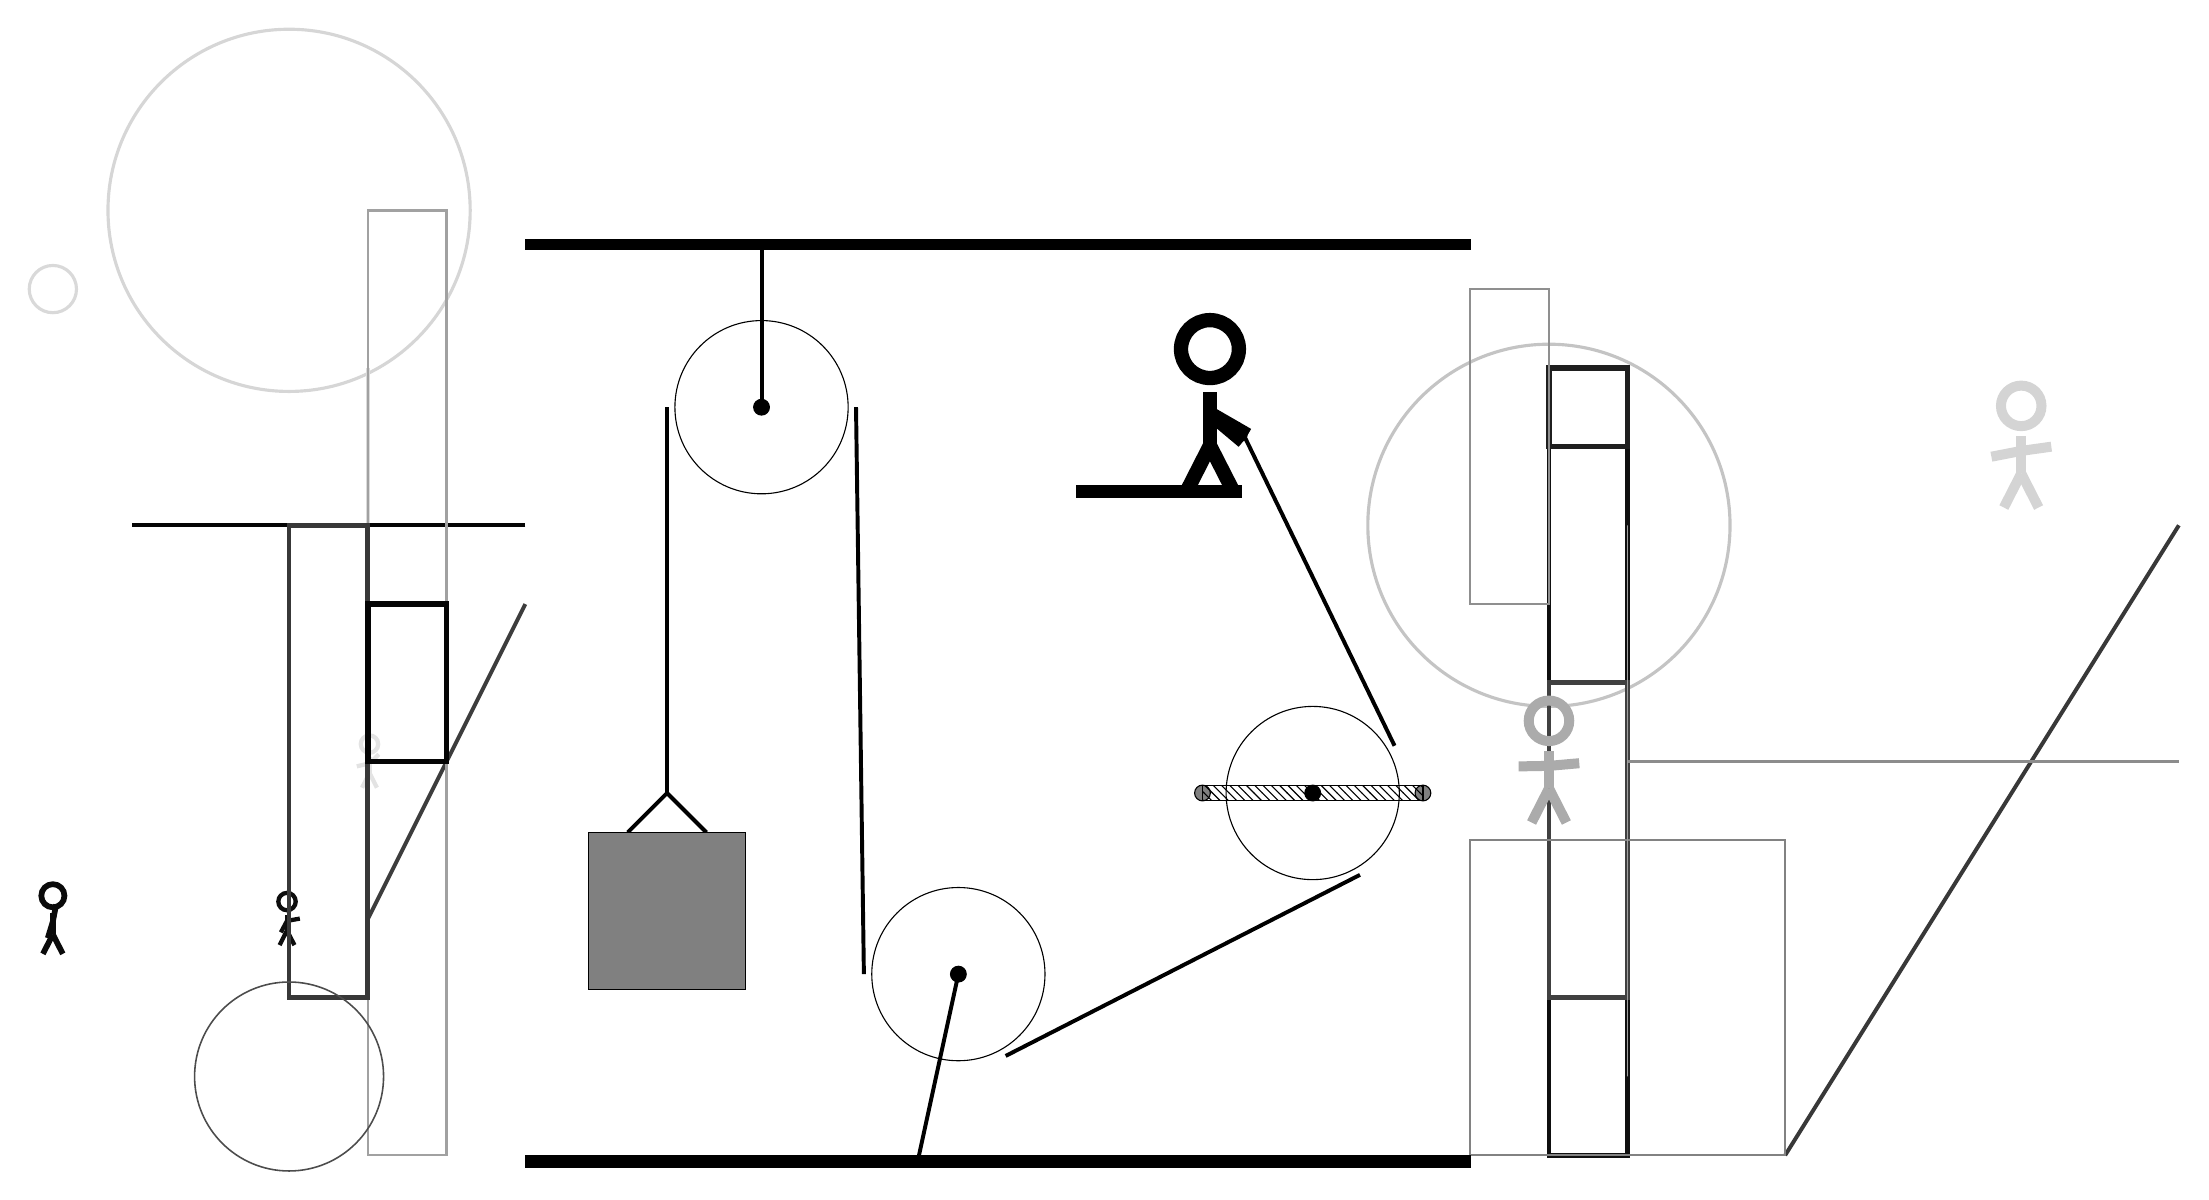
\begin{tikzpicture}
			%%%%% START %%%%%
			
			\draw[fill=black] (-2, 11.5) rectangle (10, 11.625);
			
			\draw (1, 9.5) circle (1.1);
			\draw[fill=black] (1, 9.5) circle (0.1);
			\draw[line width=0.5mm] (1, 11.5) -- (1, 9.5);
			
			\draw (3.5, 2.3) circle (1.1);
			\draw[fill=black] (3.5, 2.3) circle (0.1);
			\draw[line width=0.5mm] (3.5, 2.3) -- (3.0, 0);
			
			\draw[fill=white](8, 4.6) circle (1.1);
			\draw[fill=black] (8, 4.6) circle (0.1);
			\draw[fill=black!50] (9.4, 4.6) circle (0.1);
			\draw[fill=black!50] (6.6, 4.6) circle (0.1);
			\draw[pattern=north west lines, pattern color=black] (6.6, 4.7) rectangle (9.4, 4.5);
			
			\draw[line width=0.5mm](-0.7, 4.1) --  (-0.2, 4.6) -- (0.3, 4.1);
			\draw[fill=black!50] (-1.2, 4.1) rectangle (0.8, 2.1);
			
			\draw[line width=0.3mm, color=black!100] (10, 8) rectangle (10, 9);
			
			\node[line width=0.4mm, color=black!95] at (-5, 3) {\Strichmaxerl[3][62][10]};
			\node[line width=0.5mm, color=black!96] at (-8, 3) {\Strichmaxerl[4][73][79]};
			\draw [line width=0.4mm, color=black!23](11, 8) circle (2.3);
			\draw[line width=0.5mm, color=black!78](14, 0) -- (19, 8);
			
			\draw[line width=0.6mm, color=black!94] (11, 0) rectangle (12, 9);
			\draw[line width=0.5mm, color=black!98](-2, 8) -- (-7, 8);
			\draw[line width=0.6mm, color=black!75] (12, 6) rectangle (11, 2);
			\draw [line width=0.4mm, color=black!16](-5, 12) circle (2.3);
			\draw[line width=0.5mm, color=black!14](-4, 10) -- (-4, 8);
			\draw[line width=0.2mm, color=black!49] (10, 0) rectangle (14, 4);
			\draw[line width=0.5mm, color=black!76](-4, 3) -- (-2, 7);
			\node[line width=0.5mm, color=black!11] at (-4, 5) {\Strichmaxerl[3][13][44]};
			
			\draw[line width=0.3mm, color=black!37] (-3, 0) rectangle (-4, 12);
			\node[line width=0.5mm, color=black!33] at (11, 5) {\Strichmaxerl[7][1][5]};
			\draw[line width=0.7mm, color=black!88] (12, 9) rectangle (11, 10);
			
			\draw[line width=0.3mm, color=black!44] (11, 7) rectangle (10, 11);
			\draw[line width=0.6mm, color=black!78] (-4, 2) rectangle (-5, 8);
			\draw [line width=0.4mm, color=black!15](-8, 11) circle (0.3);
			
			\draw[line width=0.5mm, color=black!45](12, 5) -- (19, 5);
			\draw[line width=0.2mm, color=black!38] (12, 1) rectangle (12, 8);
			
			\draw [line width=0.2mm, color=black!70](-5, 1) circle (1.2);
			
			\node[line width=0.5mm, color=black!17] at (17, 9) {\Strichmaxerl[7][11][8]};
			\draw[line width=0.7mm, color=black!98] (-4, 7) rectangle (-3, 5);
			
			\draw[line width=0.5mm](-0.2, 9.5) -- (-0.2, 4.6);
			\centerarc[line width=0.5mm](1, 9.5)(180:0:1.2000000000000002)
			\draw[line width=0.5mm](2.2, 9.5) -- (2.3, 2.3);
			\centerarc[line width=0.5mm](3.5, 2.3)(180:300:1.2000000000000002);
			\draw[line width=0.5mm](4.1, 1.2608) -- (8.6, 3.5608);
			\centerarc[line width=0.5mm](8, 4.6)(300:390:1.2000000000000002);
			\draw[line width=0.5mm](9.0392, 5.2) -- (7.05, 9.3);
			
			\node at (6.75, 9.5) {\Strichmaxerl[10][-220][-30]};
			\draw[fill=black] (5, 8.5) rectangle (7.1, 8.35);
			
			\draw[fill=black] (-2, 0) rectangle (10, -0.15);
			
			%%%%% END %%%%%
		\end{tikzpicture}
	\end{figure}	
\end{document}